\documentclass{article}
\usepackage{amsmath,amssymb}
\usepackage[nomessages]{fp}% http://ctan.org/pkg/fp

\usepackage{tikz}
\usetikzlibrary{matrix,calc}
\begin{document}

\begin{align*}
M&=
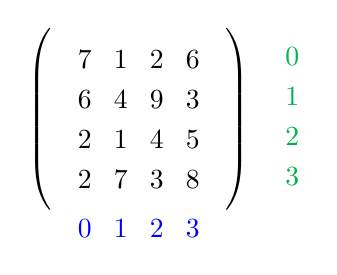
\begin{tikzpicture}[baseline=-\the\dimexpr\fontdimen22\textfont2\relax ]
\matrix(m)[matrix of math nodes,left delimiter=(,right delimiter=),inner sep=4pt,ampersand replacement=\&]
{
7 \&  1 \& 2 \&  6 \\
6 \&  4 \& 9 \&  3 \\
2 \&  1 \& 4 \&  5 \\
2 \&  7 \& 3 \&  8 \\
};
%%%%%%%%%%%%%%%%%%%%%%%%%%%%%%%%%%%%%%%
\foreach \s in {1,2,...,4}{
% bottom index
\FPeval{\result}{clip(\s-1)}%
\node[blue,shift=(m-4-\s.south),yshift=-0.4cm,text height=1ex,](0,0) {${\result}$};
}
\foreach \n in {1,2,...,4}{
\FPeval{\result}{clip(\n-1)}%
% right index
\node[green!70!blue,shift=(m-\n-4.west),xshift=1.5cm,text height=1ex,](0,0) {${\result}$} ;
}
\end{tikzpicture}
\end{align*}

\end{document}
